\begin{flushleft}
	{\color{blue!50!green}\fbox{\fontfamily{qag}\bfseries\selectfont PHẦN 1. Câu trắc nghiệm 4 phương án}}
\end{flushleft}
\setcounter{ex}{0}

\begin{ex}
Nếu hai đường tròn không cắt nhau thì số điểm chung của hai đường tròn là
\choice
{$1$}
{$2$}
{$3$}
{\True $0$}
\loigiai{
Theo định nghĩa về vị trí tương đối giữa hai đường tròn:
\begin{itemize}
    \item Hai đường tròn cắt nhau: có đúng $2$ điểm chung.
    \item Hai đường tròn tiếp xúc nhau (tiếp xúc trong hoặc tiếp xúc ngoài): có đúng $1$ điểm chung.
    \item Hai đường tròn không cắt nhau (ở ngoài nhau, đựng nhau hoặc đồng tâm): không có điểm chung nào (số điểm chung bằng $0$).
\end{itemize}
Vậy nếu hai đường tròn không cắt nhau thì số điểm chung là $0$.
\par\textbf{Chọn đáp án D.}
}
\end{ex}

\begin{ex}
Cho hai đường tròn $(O_1)$ và $(O_2)$ tiếp xúc ngoài tại $A$ và một đường thẳng $\mathrm{d}$ tiếp xúc với $(O_1)$ và $(O_2)$ lần lượt tại $B, C$. Tam giác $ABC$ là
\choice
{Tam giác cân}
{Tam giác đều}
{\True Tam giác vuông}
{Tam giác vuông cân}
\loigiai{
\begin{center}
    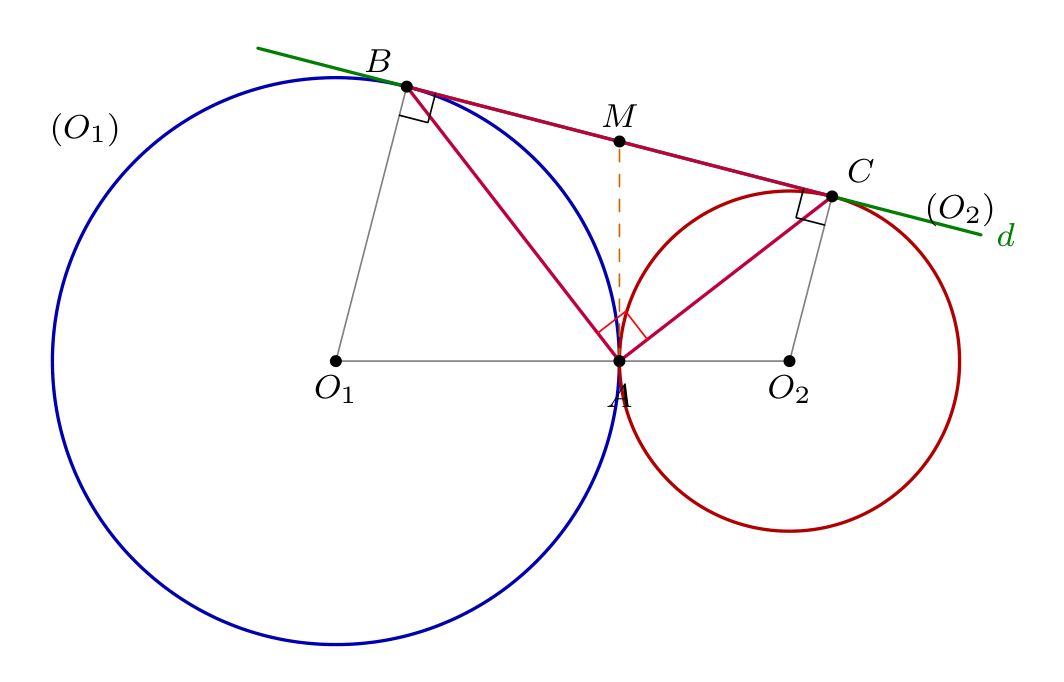
\includegraphics[width=7cm]{fig_c2.png}
\end{center}
Kẻ tiếp tuyến chung trong của hai đường tròn tại tiếp điểm $A$, tiếp tuyến này cắt đường thẳng $\mathrm{d}$ tại $M$.
Theo tính chất của hai tiếp tuyến cắt nhau:
\begin{itemize}
    \item Đối với đường tròn $(O_1)$: $MA$ và $MB$ là hai tiếp tuyến cắt nhau tại $M \Rightarrow MA = MB$.
    \item Đối với đường tròn $(O_2)$: $MA$ và $MC$ là hai tiếp tuyến cắt nhau tại $M \Rightarrow MA = MC$.
\end{itemize}
Suy ra:
$$MA = MB = MC = \dfrac{1}{2}BC$$
Tam giác $ABC$ có đường trung tuyến $AM$ ứng với cạnh $BC$ và có độ dài bằng nửa cạnh $BC$, do đó tam giác $ABC$ vuông tại $A$.
\par\textbf{Chọn đáp án C.}
}
\end{ex}

\begin{ex}
Cho đoạn thẳng $OO'$ và điểm $A$ nằm trên đoạn $OO'$ sao cho $OA = 2O'A$. Vị trí tương đối của đường tròn tâm $O$ bán kính $OA$ và đường tròn tâm $O'$ bán kính $O'A$ là
\choice
{Nằm ngoài nhau}
{Cắt nhau}
{\True Tiếp xúc ngoài}
{Tiếp xúc trong}
\loigiai{
Vì điểm $A$ nằm trên đoạn thẳng nối hai tâm $OO'$ nên:
$$OO' = OA + O'A$$
Bán kính của đường tròn tâm $O$ là $R = OA$ và bán kính của đường tròn tâm $O'$ là $R' = O'A$.
Khoảng cách giữa hai tâm là $\mathrm{d} = OO' = R + R'$.
Theo hệ thức liên hệ giữa khoảng cách hai tâm và các bán kính, điều kiện $\mathrm{d} = R + R'$ chứng tỏ hai đường tròn $(O; OA)$ và $(O'; O'A)$ tiếp xúc ngoài nhau tại điểm $A$.
\par\textbf{Chọn đáp án C.}
}
\end{ex}

\begin{ex}
Cho hai đường tròn $(O), (O')$ cắt nhau tại $A, B$ trong đó $O' \in (O)$. Kẻ đường kính $O'C$ của đường tròn $(O)$. Chọn khẳng định \textbf{sai}.
\choice
{$AC = CB$}
{$\widehat{CBO'} = 90^\circ$}
{$CA, CB$ là hai tiếp tuyến của $(O')$}
{\True $CA, CB$ là hai cát tuyến của $(O')$}
\loigiai{
\begin{center}
    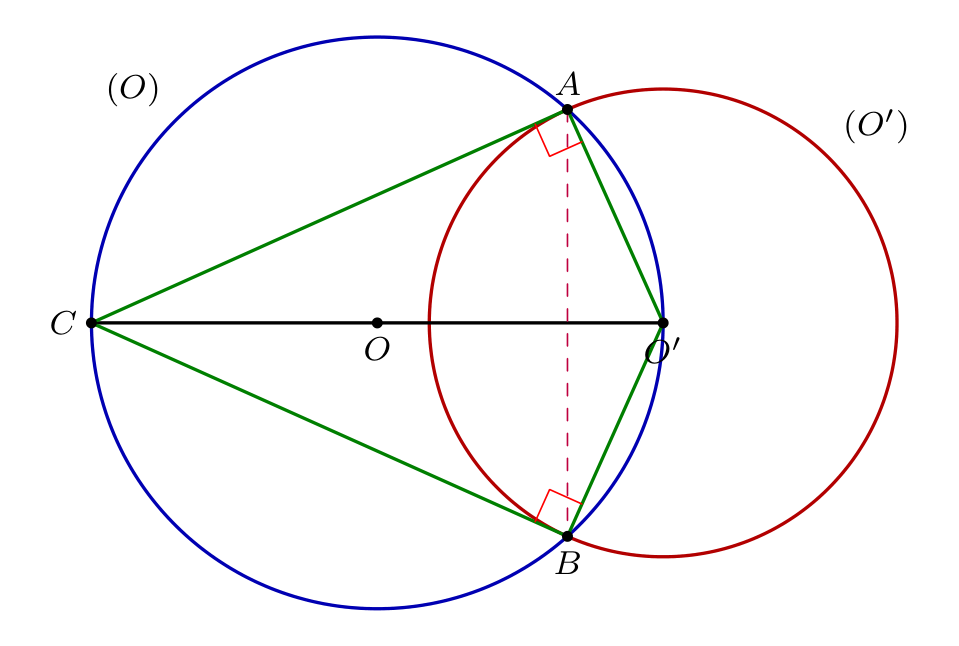
\includegraphics[width=6.5cm]{fig_c4.png}
\end{center}
Vì $O'C$ là đường kính của đường tròn $(O)$ và các điểm $A, B \in (O)$ nên:
$$\widehat{CAO'} = 90^\circ \quad \text{và} \quad \widehat{CBO'} = 90^\circ$$
(các góc nội tiếp chắn nửa đường tròn $(O)$).
\begin{itemize}
    \item Xét đường tròn $(O')$: Bán kính $O'A \perp CA$ tại $A \in (O') \Rightarrow CA$ là tiếp tuyến của $(O')$.
    \item Tương tự, bán kính $O'B \perp CB$ tại $B \in (O') \Rightarrow CB$ là tiếp tuyến của $(O')$.
\end{itemize}
Do đó $CA$ và $CB$ là hai tiếp tuyến kẻ từ $C$ đến đường tròn $(O')$, suy ra $CA = CB$ (hay $AC = CB$).
Vậy các khẳng định A, B, C đều đúng.
Khẳng định sai là D vì $CA, CB$ là hai tiếp tuyến chứ không phải hai cát tuyến.
\par\textbf{Chọn đáp án D.}
}
\end{ex}

\begin{ex}
Cho hai đường tròn tiếp xúc ngoài $(O; R)$ và $(O'; r)$ với $R > r$ và khoảng cách giữa hai tâm $OO' = \mathrm{d}$. Khi đó
\choice
{$\mathrm{d} = R - r$}
{$\mathrm{d} > R + r$}
{$R - r < \mathrm{d} < R + r$}
{\True $\mathrm{d} = R + r$}
\loigiai{
Theo bảng hệ thức vị trí tương đối giữa hai đường tròn phân biệt:
\begin{itemize}
    \item Ở ngoài nhau: $\mathrm{d} > R + r$.
    \item Tiếp xúc ngoài: $\mathrm{d} = R + r$.
    \item Cắt nhau: $R - r < \mathrm{d} < R + r$.
    \item Tiếp xúc trong: $\mathrm{d} = R - r > 0$.
    \item Đựng nhau: $\mathrm{d} < R - r$.
\end{itemize}
Do đó, khi hai đường tròn $(O; R)$ và $(O'; r)$ tiếp xúc ngoài thì $\mathrm{d} = R + r$.
\par\textit{(Ghi chú: Trong đề gốc có thể xuất hiện lỗi gõ nhầm dấu thành $\mathrm{d} < R+r$, bản chuẩn xác là $\mathrm{d} = R+r$).}
\par\textbf{Chọn đáp án D.}
}
\end{ex}

\begin{ex}
Cho đường tròn $(O_1; 3\text{ cm})$ tiếp xúc ngoài với đường tròn $(O_2; 1\text{ cm})$. Vẽ bán kính $O_1B$ và $O_2C$ song song với nhau cùng thuộc nửa mặt phẳng bờ $O_1O_2$. Gọi $D$ là giao điểm của $BC$ và $O_1O_2$. Tính số đo góc $\widehat{BAC}$ (với $A$ là tiếp điểm của $(O_1)$ và $(O_2)$).
\choice
{\True $90^\circ$}
{$60^\circ$}
{$100^\circ$}
{$80^\circ$}
\loigiai{
\begin{center}
    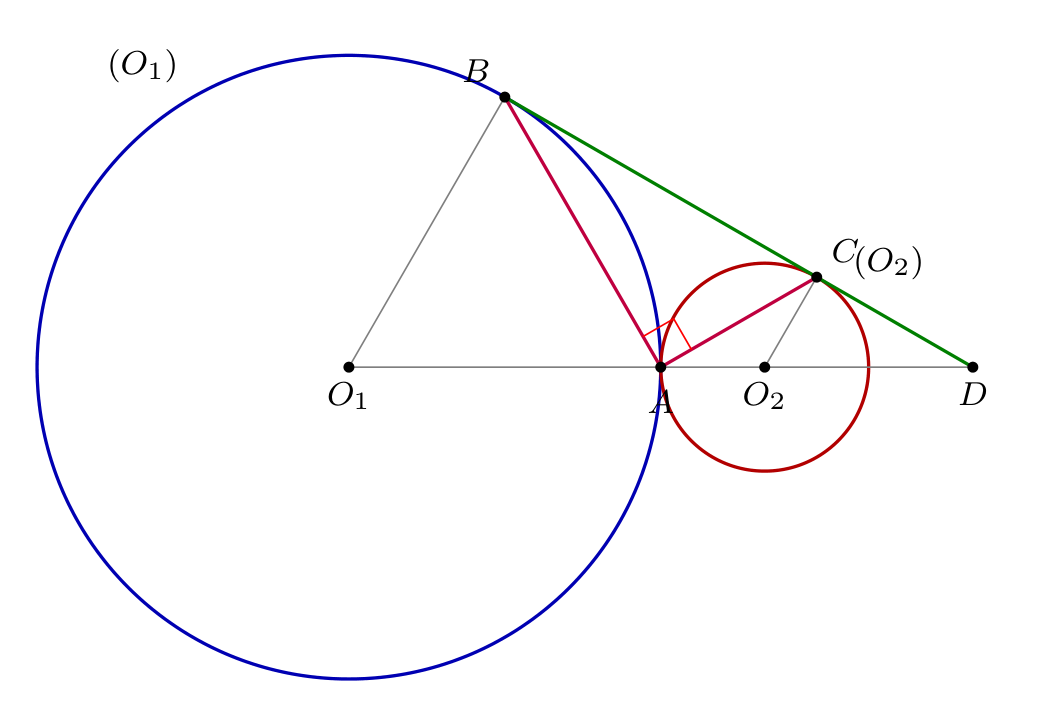
\includegraphics[width=6.5cm]{fig_c6.png}
\end{center}
Vì hai đường tròn $(O_1)$ và $(O_2)$ tiếp xúc ngoài tại $A$ nên tiếp điểm $A$ thuộc đoạn nối tâm $O_1O_2$.
Vì $O_1B \parallel O_2C$ và cùng thuộc nửa mặt phẳng bờ $O_1O_2$ nên hai góc trong cùng phía bù nhau:
$$\widehat{BO_1A} + \widehat{CO_2A} = 180^\circ$$
Xét các tam giác cân tại các tâm:
\begin{itemize}
    \item $\triangle O_1AB$ cân tại $O_1$ ($O_1A = O_1B = R_1$) $\Rightarrow \widehat{O_1AB} = \dfrac{180^\circ - \widehat{BO_1A}}{2}$.
    \item $\triangle O_2AC$ cân tại $O_2$ ($O_2A = O_2C = R_2$) $\Rightarrow \widehat{O_2AC} = \dfrac{180^\circ - \widehat{CO_2A}}{2}$.
\end{itemize}
Cộng vế với vế, ta được:
$$\widehat{O_1AB} + \widehat{O_2AC} = \dfrac{360^\circ - (\widehat{BO_1A} + \widehat{CO_2A})}{2} = \dfrac{360^\circ - 180^\circ}{2} = 90^\circ$$
Vì ba điểm $O_1, A, O_2$ thẳng hàng nên góc bẹt $\widehat{O_1AO_2} = 180^\circ$, suy ra:
$$\widehat{BAC} = 180^\circ - (\widehat{O_1AB} + \widehat{O_2AC}) = 180^\circ - 90^\circ = 90^\circ$$
\par\textbf{Chọn đáp án A.}
}
\end{ex}

\begin{ex}
Cho hai đường tròn $(O; 10\text{ cm})$ và $(O'; 5\text{ cm})$ cắt nhau tại $A, B$. Tính độ dài đoạn thẳng $OO'$ biết $AB = 8\text{ cm}$ và $O, O'$ nằm cùng phía đối với $AB$ (làm tròn kết quả đến chữ số thập phân thứ nhất).
\choice
{$OO' \approx 6{,}5\text{ cm}$}
{$OO' \approx 6{,}1\text{ cm}$}
{$OO' \approx 6{,}3\text{ cm}$}
{\True $OO' \approx 6{,}2\text{ cm}$}
\loigiai{
Gọi $H$ là giao điểm của đường nối tâm $OO'$ và dây chung $AB$.
Theo tính chất đường nối tâm của hai đường tròn cắt nhau, $OO'$ là đường trung trực của $AB$, do đó $OO' \perp AB$ tại trung điểm $H$ của $AB$:
$$AH = \dfrac{AB}{2} = \dfrac{8}{2} = 4\text{ cm}$$
Áp dụng định lý Pythagore trong các tam giác vuông $\triangle OHA$ và $\triangle O'HA$:
\begin{itemize}
    \item Trong $\triangle OHA$ vuông tại $H$:
    $$OH = \sqrt{OA^2 - AH^2} = \sqrt{10^2 - 4^2} = \sqrt{100 - 16} = \sqrt{84} \approx 9{,}165\text{ cm}$$
    \item Trong $\triangle O'HA$ vuông tại $H$:
    $$O'H = \sqrt{O'A^2 - AH^2} = \sqrt{5^2 - 4^2} = \sqrt{25 - 16} = \sqrt{9} = 3\text{ cm}$$
\end{itemize}
Vì hai tâm $O$ và $O'$ nằm cùng phía đối với dây chung $AB$ nên độ dài đoạn nối tâm $OO'$ bằng hiệu khoảng cách:
$$OO' = |OH - O'H| = \sqrt{84} - 3 \approx 9{,}165 - 3 = 6{,}165\text{ cm}$$
Làm tròn đến chữ số thập phân thứ nhất, ta được $OO' \approx 6{,}2\text{ cm}$.
\par\textit{(Ghi chú: Trong đề gốc ban đầu có sự nhầm lẫn chép số liệu $AB=24\text{ cm}$ của Câu 8 sang. Với đường tròn có bán kính $r=5\text{ cm}$, đường kính lớn nhất là $10\text{ cm}$ nên dây cung $AB$ không thể dài $24\text{ cm}$. Số liệu chuẩn mực tương ứng với đáp án là $AB = 8\text{ cm}$).}
\par\textbf{Chọn đáp án D.}
}
\end{ex}

\begin{ex}
Cho hai đường tròn $(O; 20\text{ cm})$ và $(O'; 15\text{ cm})$ cắt nhau tại $A, B$. Tính độ dài đoạn thẳng $OO'$ biết $AB = 24\text{ cm}$ và $O, O'$ nằm cùng phía đối với $AB$.
\choice
{\True $OO' = 7\text{ cm}$}
{$OO' = 8\text{ cm}$}
{$OO' = 9\text{ cm}$}
{$OO' = 25\text{ cm}$}
\loigiai{
\begin{center}
    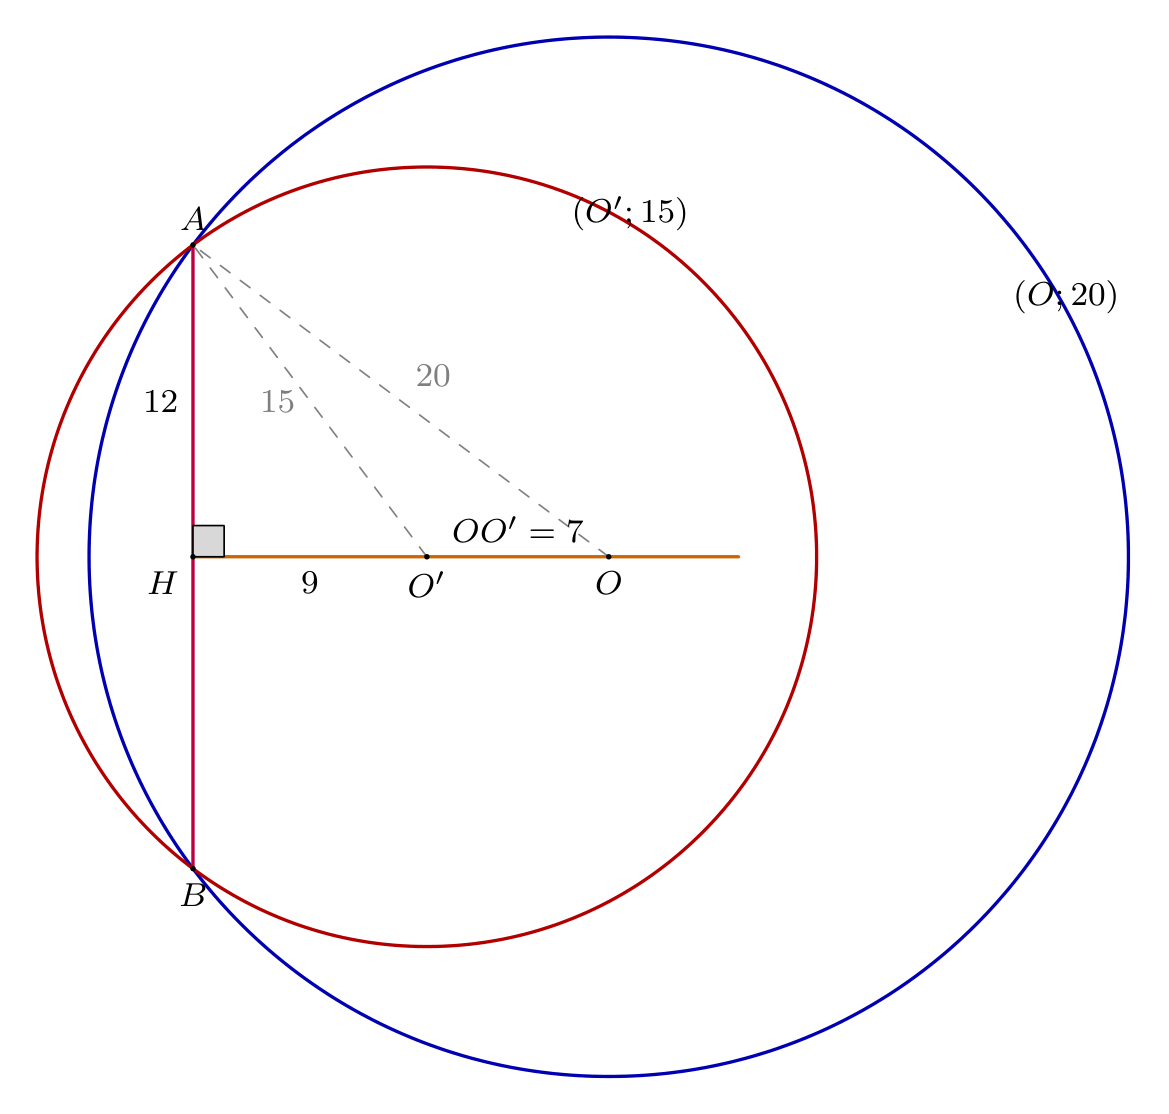
\includegraphics[width=6.5cm]{fig_c8.png}
\end{center}
Gọi $H$ là giao điểm của $OO'$ và $AB$.
Vì $OO'$ là đường trung trực của dây chung $AB$ nên $OO' \perp AB$ tại trung điểm $H$ của $AB$:
$$AH = \dfrac{AB}{2} = \dfrac{24}{2} = 12\text{ cm}$$
Áp dụng định lý Pythagore trong các tam giác vuông:
\begin{itemize}
    \item Trong $\triangle OHA$ vuông tại $H$:
    $$OH = \sqrt{OA^2 - AH^2} = \sqrt{20^2 - 12^2} = \sqrt{400 - 144} = \sqrt{256} = 16\text{ cm}$$
    \item Trong $\triangle O'HA$ vuông tại $H$:
    $$O'H = \sqrt{O'A^2 - AH^2} = \sqrt{15^2 - 12^2} = \sqrt{225 - 144} = \sqrt{81} = 9\text{ cm}$$
\end{itemize}
Vì $O$ và $O'$ nằm cùng phía đối với $AB$ nên:
$$OO' = OH - O'H = 16 - 9 = 7\text{ cm}$$
\par\textbf{Chọn đáp án A.}
}
\end{ex}

\begin{ex}
Cho hai đường tròn $(O), (O')$ tiếp xúc ngoài tại $A$. Kẻ tiếp tuyến chung ngoài $MN$ với $M \in (O), N \in (O')$. Gọi $P, Q$ lần lượt là điểm đối xứng với $M, N$ qua đường nối tâm $OO'$. Khi đó tứ giác $MNPQ$ là hình gì?
\choice
{\True Hình thang cân}
{Hình thang}
{Hình thang vuông}
{Hình bình hành}
\loigiai{
\begin{center}
    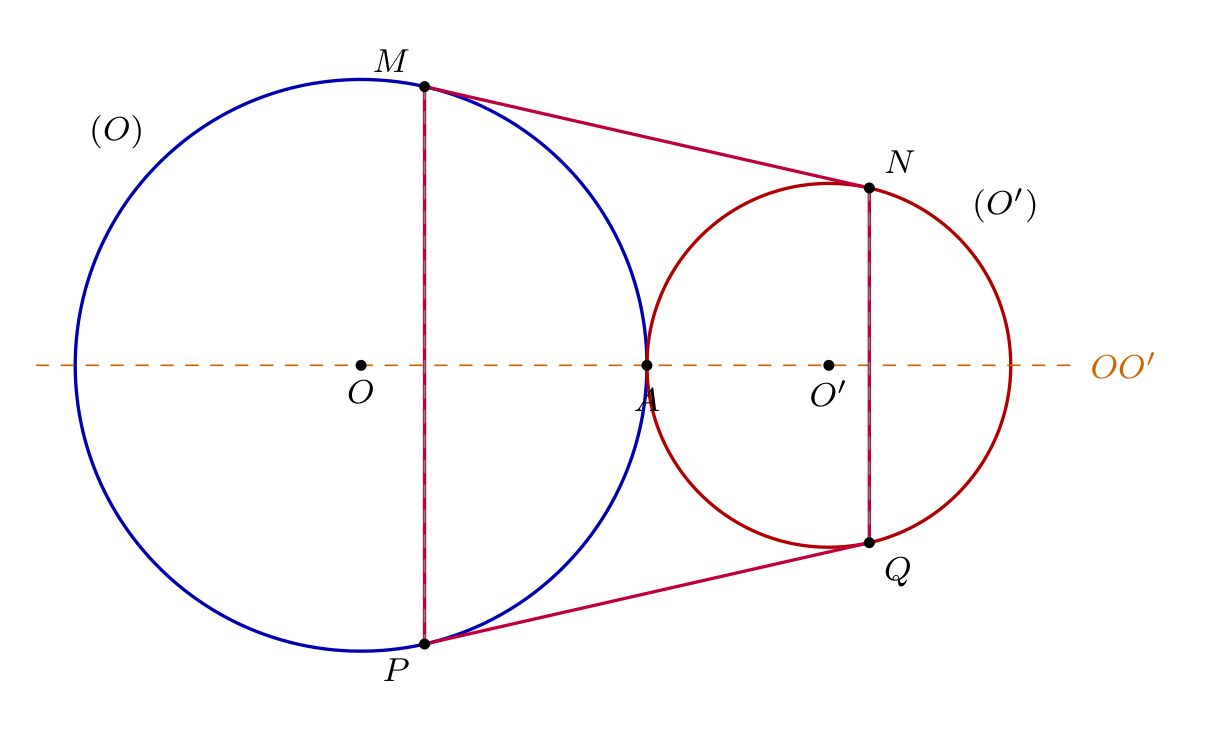
\includegraphics[width=6.5cm]{fig_c9.png}
\end{center}
Vì $P$ đối xứng với $M$ qua đường nối tâm $OO'$ nên $OO'$ là đường trung trực của đoạn thẳng $MP \Rightarrow MP \perp OO'$ và $P \in (O)$.
Tương tự, $Q$ đối xứng với $N$ qua $OO'$ nên $OO'$ là đường trung trực của $NQ \Rightarrow NQ \perp OO'$ và $Q \in (O')$.
Từ $MP \perp OO'$ và $NQ \perp OO'$ suy ra:
$$MP \parallel NQ$$
Do đó, tứ giác $MNPQ$ có hai cạnh đối song song nên là một hình thang.
Hơn nữa, phép đối xứng trục qua đường thẳng $OO'$ biến đoạn thẳng $MN$ thành đoạn thẳng $PQ$, suy ra $MN = PQ$.
Hình thang $MNPQ$ nhận đường thẳng $OO'$ làm trục đối xứng và có hai cạnh bên bằng nhau nên $MNPQ$ là \textbf{hình thang cân}.
\par\textbf{Chọn đáp án A.}
}
\end{ex}

\begin{ex}
Cho đường tròn $(O; 6\text{ cm})$ và $(O'; 2\text{ cm})$ cắt nhau tại $A, B$ sao cho $OA$ là tiếp tuyến của $(O')$. Độ dài dây chung $AB$ bằng
\choice
{$AB = 3\sqrt{10}\text{ cm}$}
{\True $AB = \dfrac{6\sqrt{10}}{5}\text{ cm}$}
{$AB = \dfrac{3\sqrt{10}}{5}\text{ cm}$}
{$AB = \dfrac{\sqrt{10}}{5}\text{ cm}$}
\loigiai{
\begin{center}
    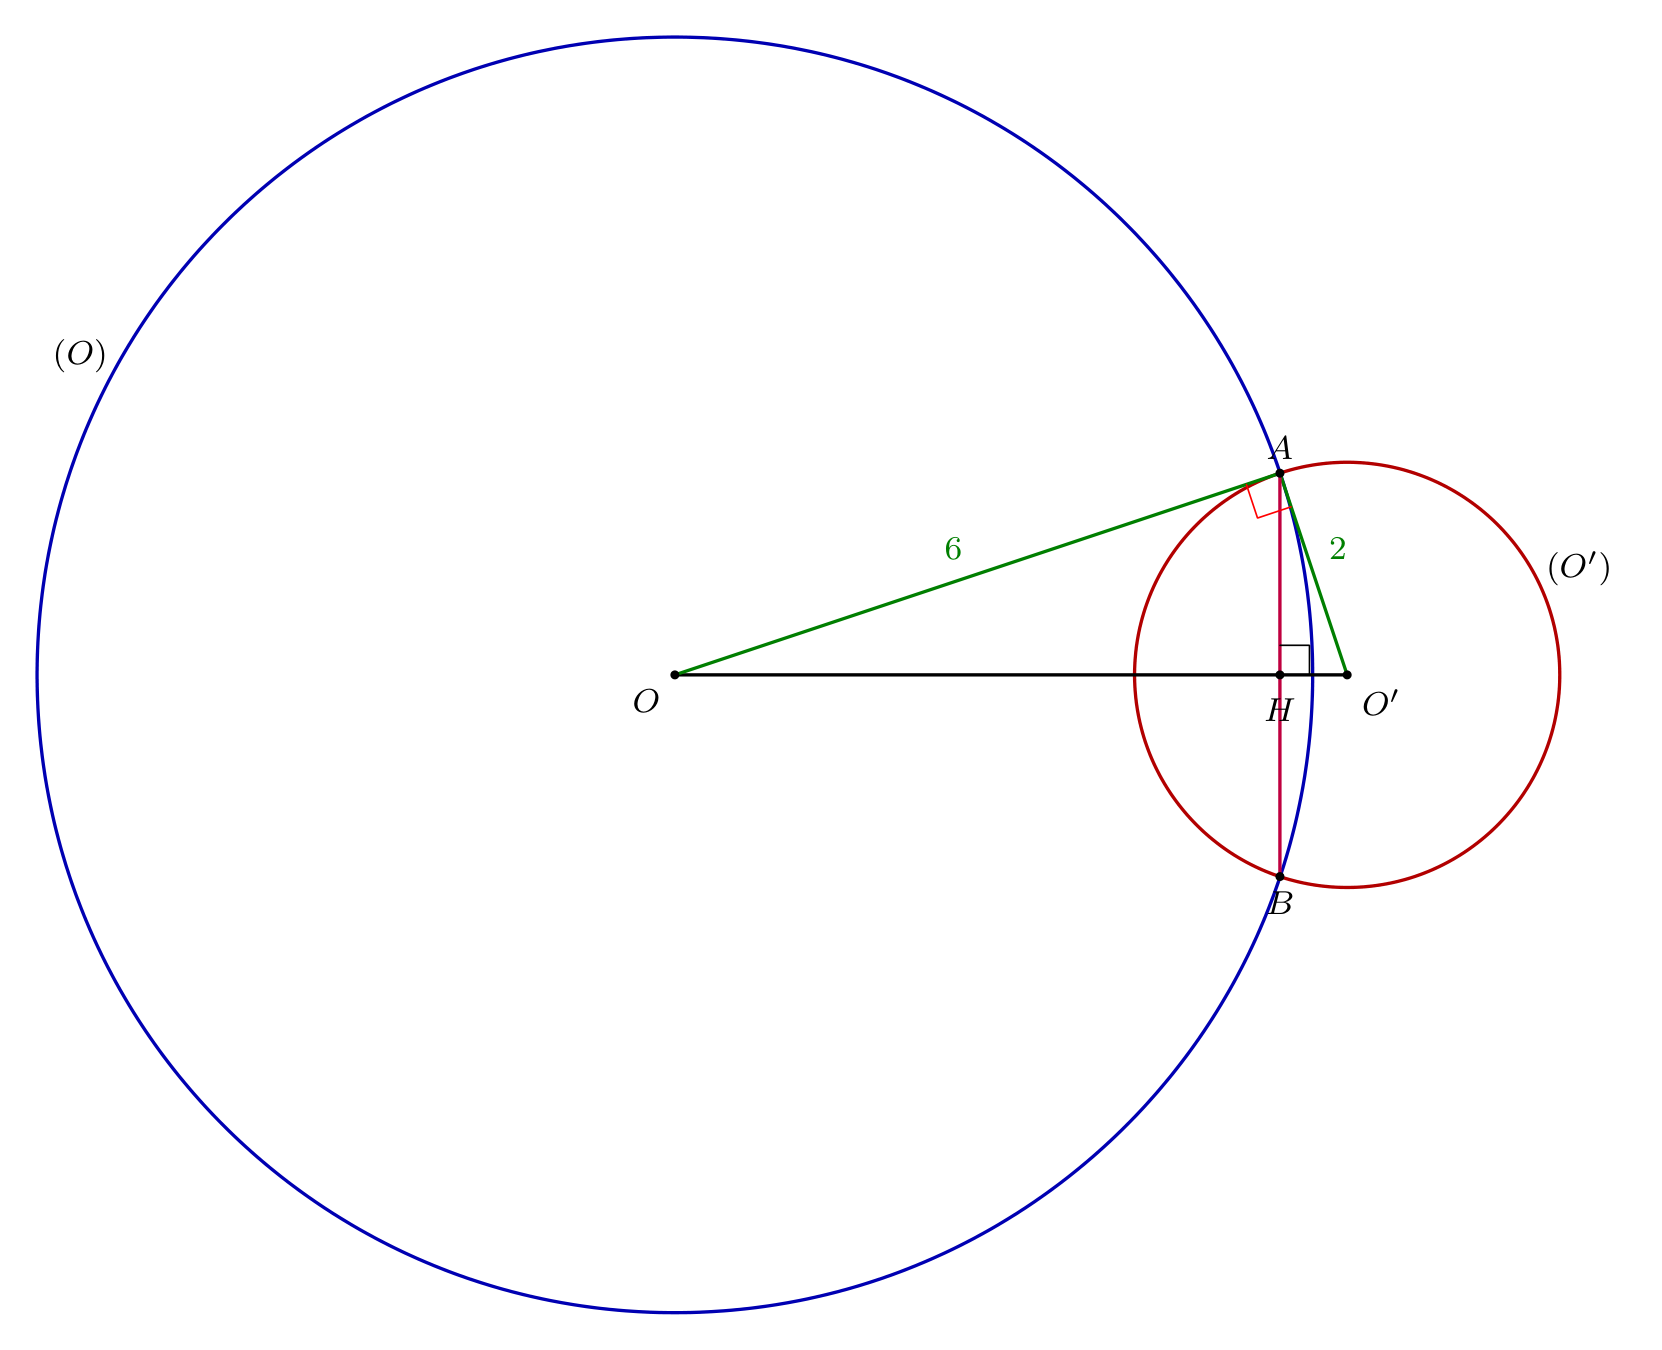
\includegraphics[width=6.5cm]{fig_c10.png}
\end{center}
Vì $OA$ là tiếp tuyến của $(O')$ tại $A$ nên $OA \perp O'A$ tại $A$.
Xét tam giác $OAO'$ vuông tại $A$, có $OA = 6\text{ cm}$, $O'A = 2\text{ cm}$.
Theo định lý Pythagore:
$$OO' = \sqrt{OA^2 + O'A^2} = \sqrt{6^2 + 2^2} = \sqrt{36 + 4} = \sqrt{40} = 2\sqrt{10}\text{ cm}$$
Gọi $H$ là giao điểm của $OO'$ và dây chung $AB$. Khi đó $OO' \perp AB$ tại trung điểm $H$ của $AB$.
Trong tam giác vuông $OAO'$, đường cao $AH$ thỏa mãn hệ thức lượng:
$$AH \cdot OO' = OA \cdot O'A \implies AH = \dfrac{OA \cdot O'A}{OO'} = \dfrac{6 \cdot 2}{2\sqrt{10}} = \dfrac{6}{\sqrt{10}} = \dfrac{3\sqrt{10}}{5}\text{ cm}$$
Do $H$ là trung điểm của $AB$ nên:
$$AB = 2AH = 2 \cdot \dfrac{3\sqrt{10}}{5} = \dfrac{6\sqrt{10}}{5}\text{ cm}$$
\par\textbf{Chọn đáp án B.}
}
\end{ex}

\begin{ex}
Cho các đường tròn $(O_1; 10\text{ cm})$, $(O_2; 15\text{ cm})$ và $(O_3; 15\text{ cm})$ tiếp xúc ngoài với nhau đôi một. Hai đường tròn $(O_2)$ và $(O_3)$ tiếp xúc nhau tại điểm $A$. Đường tròn $(O_1)$ tiếp xúc với $(O_2)$ và $(O_3)$ lần lượt tại $C$ và $B$. Khẳng định nào sau đây là đúng?
\choice
{\True $O_1A$ là tiếp tuyến chung của đường tròn $(O_2)$ và $(O_3)$}
{$O_1A = 25\text{ cm}$}
{$O_1A = 15\text{ cm}$}
{Cả A và B đều đúng}
\loigiai{
\begin{center}
    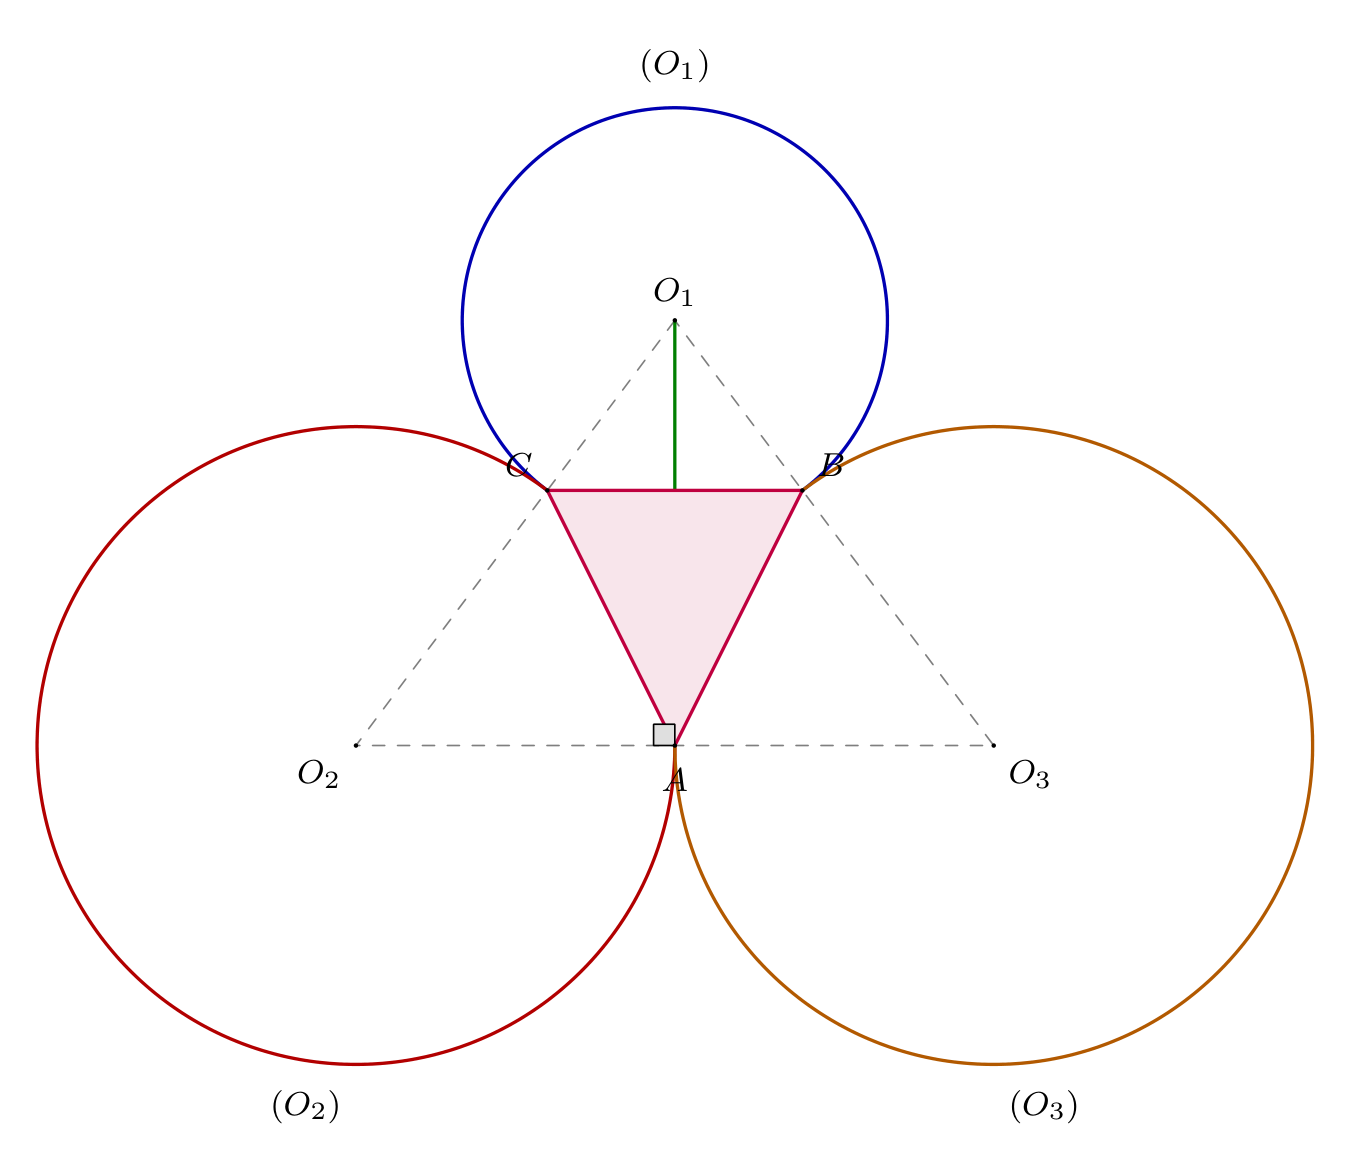
\includegraphics[width=6.5cm]{fig_c11.png}
\end{center}
Khoảng cách giữa các tâm:
\begin{itemize}
    \item $O_2O_3 = R_2 + R_3 = 15 + 15 = 30\text{ cm}$.
    \item $O_1O_2 = R_1 + R_2 = 10 + 15 = 25\text{ cm}$.
    \item $O_1O_3 = R_1 + R_3 = 10 + 15 = 25\text{ cm}$.
\end{itemize}
Vì $O_1O_2 = O_1O_3 = 25\text{ cm}$ nên $\triangle O_1O_2O_3$ cân tại $O_1$.
Điểm $A$ là tiếp điểm của $(O_2)$ và $(O_3)$ nên $O_2A = R_2 = 15\text{ cm}$ và $O_3A = R_3 = 15\text{ cm}$, suy ra $A$ là trung điểm của cạnh $O_2O_3$.
Trong tam giác cân $O_1O_2O_3$, đoạn nối đỉnh với trung điểm đáy $O_1A$ đồng thời là đường cao:
$$O_1A \perp O_2O_3 \text{ tại tiếp điểm } A$$
Vì $O_1A \perp O_2O_3$ tại tiếp điểm chung $A$ nên $O_1A$ là tiếp tuyến chung của hai đường tròn $(O_2)$ và $(O_3)$ (khẳng định A đúng).
Tính độ dài $O_1A$:
$$O_1A = \sqrt{O_1O_2^2 - O_2A^2} = \sqrt{25^2 - 15^2} = \sqrt{625 - 225} = \sqrt{400} = 20\text{ cm}$$
Vì $O_1A = 20\text{ cm} \neq 25\text{ cm}$ và $\neq 15\text{ cm}$ nên các phương án B, C, D đều sai.
\par\textbf{Chọn đáp án A.}
}
\end{ex}

\begin{ex}
Cho hai đường tròn $(O), (O')$ tiếp xúc ngoài tại $A$. Kẻ các đường kính $AB$ của $(O)$ và $AC$ của $(O')$, gọi $DE$ là tiếp tuyến chung ngoài của hai đường tròn $(D \in (O), E \in (O'))$. Gọi $M$ là giao điểm của $BD$ và $CE$. Tính diện tích tứ giác $ADME$ biết $\widehat{DOA} = 60^\circ$ và $OA = 6\text{ cm}$.
\choice
{\True $12\sqrt{3}\text{ cm}^2$}
{$12\text{ cm}^2$}
{$16\text{ cm}^2$}
{$24\text{ cm}^2$}
\loigiai{
\begin{center}
    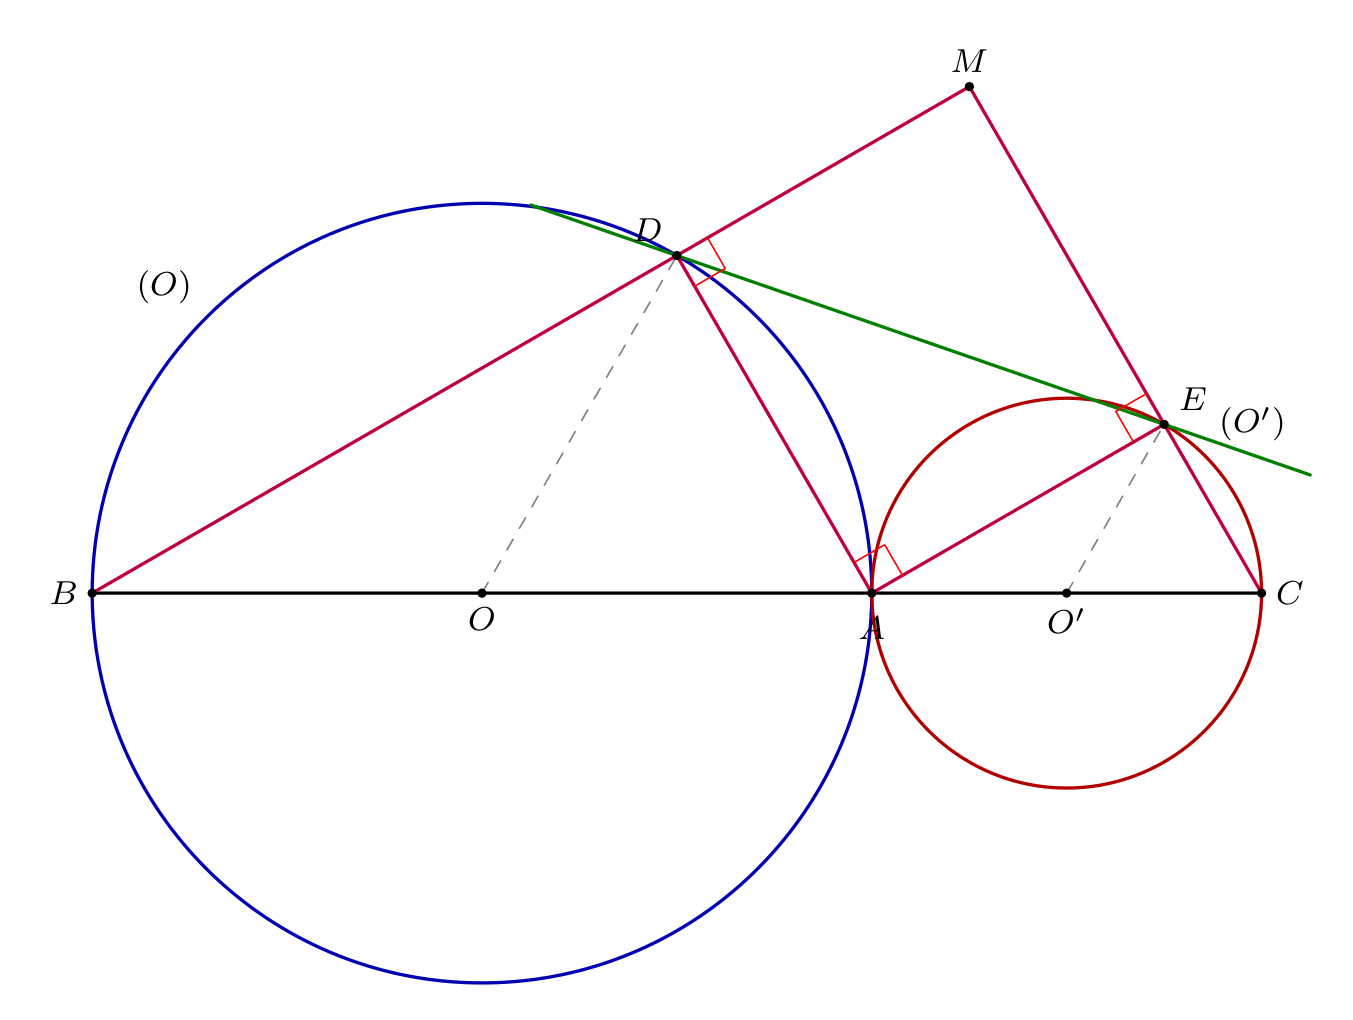
\includegraphics[width=6.5cm]{fig_c12.png}
\end{center}
Vì $AB$ là đường kính của $(O)$ nên $\widehat{ADB} = 90^\circ$ (góc nội tiếp chắn nửa đường tròn) $\Rightarrow AD \perp BD$ tại $D$, hay $\widehat{ADM} = 90^\circ$.
Tương tự, $AC$ là đường kính của $(O')$ nên $\widehat{AEC} = 90^\circ \Rightarrow AE \perp CE$ tại $E$, hay $\widehat{AEM} = 90^\circ$.
Lại có $DE$ là tiếp tuyến chung ngoài của hai đường tròn tiếp xúc ngoài tại $A$, theo tính chất tiếp tuyến chung:
$$\widehat{DAE} = 90^\circ$$
Tứ giác $ADME$ có ba góc vuông ($\widehat{DAE} = \widehat{ADM} = \widehat{AEM} = 90^\circ$) nên là một \textbf{hình chữ nhật}.
Diện tích hình chữ nhật $ADME$ là:
$$S_{ADME} = AD \cdot AE$$
Xét tam giác $OAD$: Ta có $OA = OD = R = 6\text{ cm} \Rightarrow \triangle OAD$ cân tại $O$.
Mà $\widehat{DOA} = 60^\circ$ nên $\triangle OAD$ là tam giác đều:
$$AD = OA = 6\text{ cm} \quad \text{và} \quad \widehat{ODA} = 60^\circ$$
Vì $DE$ là tiếp tuyến của $(O)$ tại $D$ nên $OD \perp DE$, do đó:
$$\widehat{ADE} = 90^\circ - \widehat{ODA} = 90^\circ - 60^\circ = 30^\circ$$
Trong tam giác vuông $ADE$ tại $A$:
$$AE = AD \cdot \tan \widehat{ADE} = 6 \cdot \tan 30^\circ = 6 \cdot \dfrac{1}{\sqrt{3}} = 2\sqrt{3}\text{ cm}$$
Vậy diện tích hình chữ nhật $ADME$ là:
$$S_{ADME} = AD \cdot AE = 6 \cdot 2\sqrt{3} = 12\sqrt{3}\text{ cm}^2$$
\par\textbf{Chọn đáp án A.}
}
\end{ex}

\begin{ex}
Cho hai đường tròn $(O), (O')$ tiếp xúc ngoài tại $A$. Kẻ các đường kính $AB$ của $(O)$ và $AC$ của $(O')$, gọi $DE$ là tiếp tuyến chung ngoài của hai đường tròn $(D \in (O), E \in (O'))$. Gọi $M$ là giao điểm của $BD$ và $CE$. Tính diện tích tứ giác $ADME$ biết $\widehat{DOA} = 60^\circ$ và $OA = 8\text{ cm}$.
\choice
{$12\sqrt{3}\text{ cm}^2$}
{\True $\dfrac{64\sqrt{3}}{3}\text{ cm}^2$}
{$\dfrac{32\sqrt{3}}{3}\text{ cm}^2$}
{$36\text{ cm}^2$}
\loigiai{
Chứng minh tương tự Câu 12:
Tứ giác $ADME$ là hình chữ nhật.
Tam giác $OAD$ cân tại $O$ và có $\widehat{DOA} = 60^\circ$ nên là tam giác đều, suy ra:
$$AD = OA = 8\text{ cm} \quad \text{và} \quad \widehat{ODA} = 60^\circ$$
Vì $OD \perp DE$ nên:
$$\widehat{ADE} = 90^\circ - \widehat{ODA} = 90^\circ - 60^\circ = 30^\circ$$
Trong tam giác vuông $ADE$ tại $A$:
$$AE = AD \cdot \tan 30^\circ = 8 \cdot \dfrac{\sqrt{3}}{3} = \dfrac{8\sqrt{3}}{3}\text{ cm}$$
Vậy diện tích hình chữ nhật $ADME$ là:
$$S_{ADME} = AD \cdot AE = 8 \cdot \dfrac{8\sqrt{3}}{3} = \dfrac{64\sqrt{3}}{3}\text{ cm}^2$$
\par\textbf{Chọn đáp án B.}
}
\end{ex}

\begin{ex}
Cho các đường tròn $(O_1; 10\text{ cm})$, $(O_2; 15\text{ cm})$ và $(O_3; 15\text{ cm})$ tiếp xúc ngoài với nhau đôi một. Hai đường tròn $(O_2)$ và $(O_3)$ tiếp xúc nhau tại điểm $A$. Đường tròn $(O_1)$ tiếp xúc với $(O_2)$ và $(O_3)$ lần lượt tại $C$ và $B$. Tính diện tích tam giác $ABC$.
\choice
{$36\text{ cm}^2$}
{\True $72\text{ cm}^2$}
{$144\text{ cm}^2$}
{$96\text{ cm}^2$}
\loigiai{
Chọn hệ trục tọa độ vuông góc $Oxy$ với gốc đặt tại tiếp điểm $A(0; 0)$ trên đường nối tâm $O_2O_3$:
\begin{itemize}
    \item Trục hoành $Ox$ trùng với đường nối tâm $O_2O_3$, khi đó $O_2(-15; 0)$ và $O_3(15; 0)$.
    \item Trục tung $Oy$ vuông góc với $O_2O_3$ tại $A$, đi qua tâm $O_1$.
\end{itemize}
Vì $O_1O_2 = R_1 + R_2 = 10 + 15 = 25\text{ cm}$ nên tung độ của điểm $O_1$ là:
$$y_{O_1} = \sqrt{O_1O_2^2 - O_2A^2} = \sqrt{25^2 - 15^2} = \sqrt{400} = 20 \implies O_1(0; 20)$$
Tìm tọa độ các tiếp điểm:
\begin{itemize}
    \item Điểm $C$ thuộc đoạn thẳng $O_2O_1$ và chia đoạn $O_2O_1$ theo tỉ số $\dfrac{O_2C}{O_2O_1} = \dfrac{15}{25} = \dfrac{3}{5}$:
    $$x_C = x_{O_2} + \dfrac{3}{5}(x_{O_1} - x_{O_2}) = -15 + \dfrac{3}{5}(0 - (-15)) = -6$$
    $$y_C = y_{O_2} + \dfrac{3}{5}(y_{O_1} - y_{O_2}) = 0 + \dfrac{3}{5}(20 - 0) = 12 \implies C(-6; 12)$$
    \item Tương tự, điểm $B$ thuộc đoạn thẳng $O_3O_1$ chia đoạn $O_3O_1$ theo tỉ số $\dfrac{O_3B}{O_3O_1} = \dfrac{3}{5}$:
    $$x_B = x_{O_3} + \dfrac{3}{5}(x_{O_1} - x_{O_3}) = 15 + \dfrac{3}{5}(0 - 15) = 6$$
    $$y_B = y_{O_3} + \dfrac{3}{5}(y_{O_1} - y_{O_3}) = 0 + \dfrac{3}{5}(20 - 0) = 12 \implies B(6; 12)$$
\end{itemize}
Tam giác $ABC$ có các đỉnh $A(0; 0)$, $B(6; 12)$, $C(-6; 12)$:
\begin{itemize}
    \item Cạnh đáy $BC$ nằm ngang trên đường thẳng $y = 12$, có độ dài $BC = x_B - x_C = 6 - (-6) = 12\text{ cm}$.
    \item Chiều cao $h$ hạ từ đỉnh $A(0; 0)$ đến đường thẳng chứa cạnh $BC$ ($y = 12$) là $h = 12\text{ cm}$.
\end{itemize}
Diện tích tam giác $ABC$ là:
$$S_{\triangle ABC} = \dfrac{1}{2} \cdot BC \cdot h = \dfrac{1}{2} \cdot 12 \cdot 12 = 72\text{ cm}^2$$
\par\textbf{Chọn đáp án B.}
}
\end{ex}

\begin{ex}
Cho hai đường tròn $(O; R)$ và $(O'; r)$ với $R > r$ tiếp xúc ngoài tại $A$. Vẽ các bán kính $OB \parallel O'D$ với $B, D$ cùng thuộc nửa mặt phẳng bờ $OO'$. Đường thẳng $DB$ và $OO'$ cắt nhau tại $I$. Tiếp tuyến chung ngoài $GH$ của $(O)$ và $(O')$ với $G, H$ nằm ở nửa mặt phẳng bờ $OO'$ không chứa $B, D$. Tính $OI$ theo $R$ và $r$.
\choice
{$OI = \dfrac{R+r}{R-r}$}
{$OI = \dfrac{R-r}{R+r}$}
{$OI = \dfrac{R(R-r)}{R+r}$}
{\True $OI = \dfrac{R(R+r)}{R-r}$}
\loigiai{
\begin{center}
    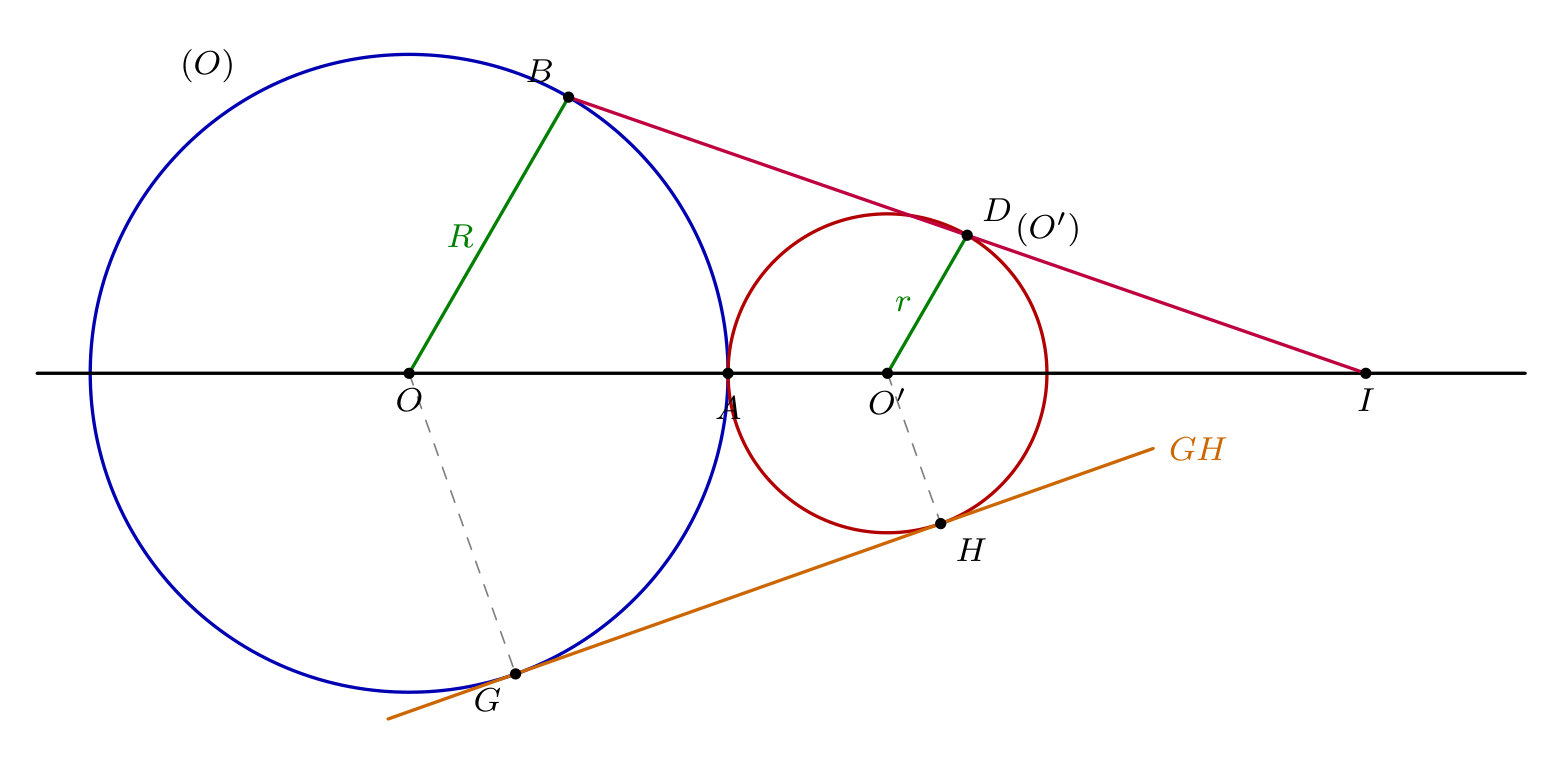
\includegraphics[width=6.5cm]{fig_c15.png}
\end{center}
Xét tam giác $IOB$ có $O'D \parallel OB$ ($D \in IB, O' \in IO$).
Theo định lý Ta-lét trong tam giác:
$$\dfrac{IO'}{IO} = \dfrac{O'D}{OB} = \dfrac{r}{R}$$
Do hai đường tròn $(O; R)$ và $(O'; r)$ tiếp xúc ngoài tại $A$ nên khoảng cách hai tâm là:
$$OO' = OA + O'A = R + r$$
Mặt khác, vì $R > r$ nên điểm $O'$ nằm giữa hai điểm $I$ và $O$, ta có:
$$IO - IO' = OO' = R + r$$
Từ $\dfrac{IO'}{IO} = \dfrac{r}{R}$, áp dụng tính chất của dãy tỉ số bằng nhau:
$$\dfrac{IO - IO'}{IO} = \dfrac{R - r}{R}$$
Thay $IO - IO' = R + r$ vào hệ thức:
$$\dfrac{R + r}{OI} = \dfrac{R - r}{R} \implies OI = \dfrac{R(R + r)}{R - r}$$
\par\textbf{Chọn đáp án D.}
}
\end{ex}

\vspace{0.4cm}
\begin{center}
\textbf{BẢNG ĐÁP ÁN TRẮC NGHIỆM} \\[0.2cm]
\begin{tabular}{|c|c|c|c|c|c|c|c|c|c|c|c|c|c|c|}
\hline
\textbf{1} & \textbf{2} & \textbf{3} & \textbf{4} & \textbf{5} & \textbf{6} & \textbf{7} & \textbf{8} & \textbf{9} & \textbf{10} & \textbf{11} & \textbf{12} & \textbf{13} & \textbf{14} & \textbf{15} \\
\hline
\textbf{D} & \textbf{C} & \textbf{C} & \textbf{D} & \textbf{D} & \textbf{A} & \textbf{D} & \textbf{A} & \textbf{A} & \textbf{B} & \textbf{A} & \textbf{A} & \textbf{B} & \textbf{B} & \textbf{D} \\
\hline
\end{tabular}
\end{center}

\vspace{0.3cm}
\begin{center}
\textbf{--- HẾT ---}
\end{center}

